\documentclass{article} % for thesis

% \usepackage[top=0.5in, bottom=0.5in, left=0.5in, right=0.5in]{geometry}
% \documentclass[twocolumn,9pt]{article}
\usepackage{spconf}
\usepackage[utf8]{inputenc}
\usepackage{natbib}
\usepackage{graphicx}
\usepackage{stfloats} % for positioning of figure* on the same page
\usepackage{caption}
\usepackage{tikz}
\usepackage[inline]{enumitem}
\usepackage{amsmath}
\usepackage{subcaption}
\usepackage[breaklinks=true,colorlinks=true, allcolors=blue]{hyperref}
\usepackage{breakcites}
\usepackage{microtype}
\usepackage{lipsum}
\usepackage{xcolor}
\usepackage{array}
\usepackage{float}
\usepackage{adjustbox}
\usepackage{listings}
\usepackage{csquotes}
\usepackage{makecell}
\usepackage{pdfpages}
\usepackage{xspace}


% to do:
% a few more scenarios
% hearing tests
% one other way to present results is grouped by which losses are most appropriate for each situtation

\usepackage{xcolor}
\usepackage[utf8]{inputenc}       % For UTF-8 encoding
\usepackage{listings}
\usepackage{amsmath}              % Optional: for math symbols

\lstdefinelanguage{Faust}{
    morekeywords={import, process, environment, declare, with, if, else, while, for, int, float, true, false},
    sensitive=true,
    morecomment=[l]{//}, % Line comment
    morecomment=[s]{/*}{*/}, % Block comment
    morestring=[b]", % Strings
}

% Customize the appearance of the code
\lstset{
    language=Faust,
    backgroundcolor=\color{lightgray!20},
    basicstyle=\ttfamily\small,
    keywordstyle=\color{blue}\bfseries,
    stringstyle=\color{orange},
    commentstyle=\color{green}\itshape,
    showstringspaces=false,
    numbers=left,
    numberstyle=\tiny,
    frame=single,
    breaklines=true,
      basicstyle=\ttfamily,
  % literate={\delta}{{\(\delta\)}},
}


\captionsetup[lstlisting]{justification=centering, singlelinecheck=false}
\providecommand{\gls}[1]{#1}
\newcommand{\highlight}[1]{\textcolor[RGB]{00,150,00}{#1}}
\newcommand{\todo}[1]{\textcolor{red}{#1}}

\newcommand{\SIMSESpec}{\texttt{SIMSE\_Spec}\xspace}
\newcommand{\LoneSpec}{\texttt{L1\_Spec}\xspace}
\newcommand{\JTFS}{\texttt{JTFS}\xspace}
\newcommand{\DTWEnv}{\texttt{DTW\_Envelope}\xspace}
\newcommand{\OutDomain}{\textbf{Out-Domain Generation}\xspace}

\newcommand{\BPNoise}{\textbf{BP-Noise}\xspace}
\newcommand{\BPSaw}{\textbf{BP-Saw}\xspace}
\newcommand{\AddSineSaw}{\textbf{Add-SineSaw}\xspace}
\newcommand{\AmpMod}{\textbf{Noise-AM}\xspace}
\newcommand{\FMMod}{\textbf{SineSaw-AM}\xspace}
\newcommand{\FMModvtwo}{\textbf{SineSine-AM}\xspace}
\newcommand{\PitchBendUp}{\textbf{PitchBend-Up}\xspace}

\title{Selecting Loss Functions for Out-of-Domain Sound-Matching}
\begin{document}

\author{Amir Salimi, Abram Hindle, Osmar R. Za{\"i}ane}

% \name{Amir Salimi, Abram Hindle, Osmar R. Za{\"i}ane}
% \address{University of Alberta}

\maketitle

\begin{abstract}
    Out-of-domain sound-matching refers to automatically programming a synthesizer towards a sound that it cannot accurately replicate. Measuring performance in out-of-domain sound-matching is a difficult task due reasons such as the subjective experience of sound, open-set recognition, etc. Here we present a series of out-of-domain tasks using four loss functions and synthesizers with non-overlapping functionalities. The experiments here are designed such that differences in parameters (whether all parameters or a subset) are well suited for measuring performance in sound-matching. The out-of-domain experiments here confirm that the success of loss functions is highly dependent on the method of synthesis and the target sound. 
\end{abstract}

\section{Introduction}
Audio synthesizers are music instruments which utilize digital signal processing functions for the creation of sound. Synthesizers have different characteristics depending on which functions they utilize, and which parameters are given to those functions. One method of sound-design with a synthesizer involves the continual listening and modification of the parameters to approximate output sounds which have the desired characteristics of the target sound. Sound-matching is the task of automation this process.  

Here, the target sound can be any sound that the sound-designer finds interesting or inspiring. A major discrepancy in past works in sound-matching and the process it aims to automate is that the target sounds are from sources other than the synthesizer itself (or out-of-domain) and the goal is not the replication of the sound, but imitation of a particular characteristic. The overwhelming majority of current literature on sound-matching has been centered around in-domain replication of sounds, where the target sound is the output of the synthesizer itself, and performance is measured by whether or not the target sound and the synthesizer's output are identical. 

Defining success in out-of-domain sound-matching is difficult, as the goal becomes imitation of a subset of the target sound's characteristics. This issue calls for similarity metrics (or loss functions) which measure the similarity of those particular characteristics of interest. 


In a previous work, we presented a number of sound-matching experiments which suggest that the selection of the best performing loss functions for sound-matching is highly dependent on the method of synthesis~\cite{salimi2025soundmatching}. Much like the majority of previous works in sound-matching, the experiments were in-domain, that is, the synthesizer is capable of perfect replication of the target sound (usually, the target sound is made by the synthesizer itself). We noted the lack of out-of-domain experiments as a weakness not only in our previous work, but in the field of sound-matching as a whole. Here, we present a number of sound-matching experiments where the synthesizers are not capable of complete replication of the target sound. 

\section{Motivation}


\begin{figure}[htbp]
    \centering
    \begin{subfigure}[b]{0.45\linewidth}
        \centering
        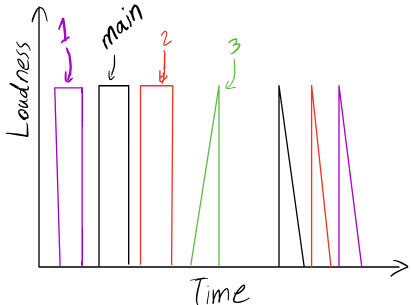
\includegraphics[width=\linewidth]{images/ood_motivation_time_alignment_doodle.png}
        \caption{}
        \label{fig:sub1}
    \end{subfigure}
    \hspace{0.05\linewidth}
    \begin{subfigure}[b]{0.45\linewidth}
        \centering
        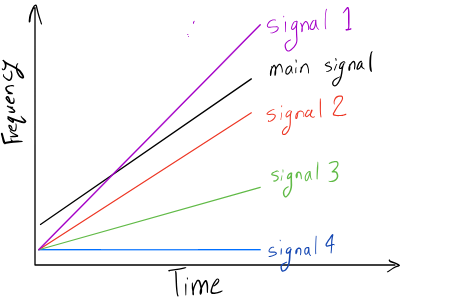
\includegraphics[width=\linewidth]{images/ood_motivation_frequency_alignment_doodle.png}
        \caption{Second image.}
        \label{fig:sub2}
    \end{subfigure}
    \caption{Two side-by-side images.}
    \label{fig:twoside}
\end{figure}

\section{Experiment Setup}
\label{sec:experiment_setup}
% loss functions, target vs imitator, training loop
For each combination of synthesizer program and loss function, 300 sound-matching experiments are conducted and the automatic evaluation evaluation values are recorded after 200 iterations of the sound-matching loop. From the 300 targets and outputs, we select 40 examples for manual ranking. 


\section{Out-of-Domain Examples}
We look at some examples of out-of-domain sound-matching experiments, discuss the evaluation methods, and analyze the loss function landscapes. 

\subsection{Band Pass Matching}
In this scenario, the two synthesizers are the application of band-passing to noise (\BPNoise) and saw waves (\BPSaw). Examples of these programs are given in Listings~\ref{lst:program0} and ~\ref{lst:program0_saw} respectively. Previously, we've seen that with in-domain sound-matching of \BPNoise, the loss functions utilizing spectrogram differences were the best performers, and speculated that this was related to the clear visibility of filter-cutoffs in a spectrogram. 
 
 Here we use \BPSaw as the target synthesizer, and \BPNoise as the imitator. We define success in sound-matching here as the proximity of the imitator's high and low-pass cutoffs to that of the target. This allows for P-Loss to become an objective measure of success. With this objective, we see that \SIMSESpec is once again the clear best performing loss function.

 \begin{figure*}[htbp]
  \centering
  % 1st row
    \begin{minipage}{\textwidth}
      % left‐column labels
      \begin{minipage}{0.03\textwidth}
        \footnotesize\raggedleft
        \vspace{0.5cm}
        SIMSE\\[0.6cm]
        L1\\[0.65cm]
        JTFS\\[0.65cm]
        DTW
      \end{minipage}%
      \begin{minipage}{0.96\textwidth}\centering
        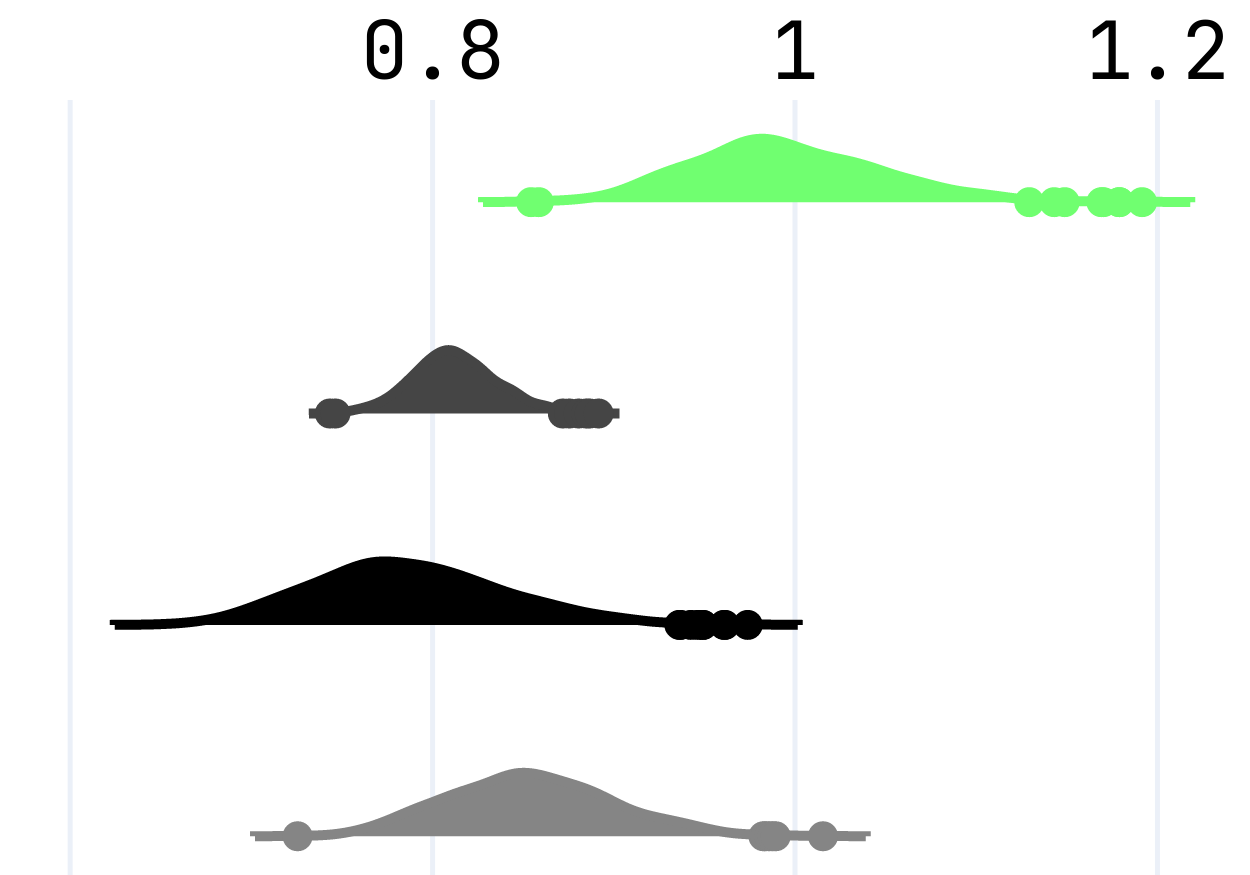
\includegraphics[width=0.45\textwidth]{images/npsk_ood_P_Loss_3.png}%
        \hspace{0.03\textwidth}%
      \end{minipage}
    \end{minipage}
     \caption{Bootstrapped distributions and ranks for band-pass sound matching.}
  \label{fig:npsk_BP}
  
\end{figure*}
 


\begin{lstlisting}[caption={\BPNoise}, label={lst:program0}, language=Faust,
                  float, floatplacement=!H, xleftmargin=1em, xrightmargin=0.5em, firstnumber=0, aboveskip=0em, belowskip=-1em]
import("stdfaust.lib");
lp_cut = hslider("lp_cut",900,100,5000,5);
hp_cut = hslider("hp_cut",100,1,400,5);
process = no.noise:fi.lowpass(3,lp_cut):fi.highpass(10,hp_cut);
\end{lstlisting}

\begin{lstlisting}[caption={\BPSaw}, label={lst:program0_saw}, language=Faust,
                  float, floatplacement=!H, xleftmargin=1em, xrightmargin=0.5em, firstnumber=0, aboveskip=0em, belowskip=-1em]
import("stdfaust.lib");
lp_cut = hslider("lp_cut", 2801, 100, 5000, 1);
hp_cut = hslider("hp_cut", 142, 1, 400, 1);
sawOsc(f) = +(f/ma.SR) ~ ma.frac;
process = sawOsc(30):fi.lowpass(5, lp_cut):fi.highpass(5, hp_cut);
\end{lstlisting}


\subsection{AM-Synthesizer Matching}
\begin{lstlisting}[caption={\FMMod}, label={lst:program3},language=Faust,float,floatplacement=!H,xleftmargin=1em,xrightmargin=0.5em,firstnumber=0,aboveskip=0em, belowskip=-1em]
import("stdfaust.lib");
carrier = hslider("carrier",car_a,car_b,car_c,1);
amp = hslider("amp",amp_a,amp_b,amp_c,1);
sineOsc(f) = +(f/ma.SR) ~ ma.frac:*(2*ma.PI) : sin;
sawOsc(f) = +(f/ma.SR) ~ ma.frac;
process = sineOsc(amp)*sawOsc(carrier);
\end{lstlisting}


\begin{lstlisting}[caption={\FMModvtwo}, label={lst:program3_v2},language=Faust,float,floatplacement=!H,xleftmargin=1em,xrightmargin=0.5em,firstnumber=0,aboveskip=0em, belowskip=-1em]
import("stdfaust.lib");
carrier = hslider("carrier",car_a,car_b,car_c,1);
amp = hslider("amp",amp_a,amp_b,amp_c,1);
sineOsc(f) = +(f/ma.SR) ~ ma.frac:*(2*ma.PI) : sin;
process = sineOsc(amp)*sineOsc(carrier);
\end{lstlisting}
\label{sec:am_sound_matching}
We try out three different scenarios of out-of-domain sound-matching with AM-Synthesizers. \FMMod is described in Listing~\ref{lst:program3} and \FMModvtwo described in Listing~\ref{lst:program3_v2} are the basis of the three variations of these experiments. \FMMod generates a sound by modifying the amplitude of a saw oscillator with a sinusoidal LFO. \FMModvtwo is a modification which uses sine oscillators for both the carrier and the modulator. In this section, we will refer to the LFO frequency as \texttt{amp} and carrier frequency as \texttt{car}. The value of \texttt{amp} shapes the amplitude of the sound (or the wobbling effect), and \texttt{car} determines the frequency of the sound.

In these scenarios, the \texttt{amp} values can match, but the frequency content cannot, either because the range of available frequencies are different (scenario 1) or the imitator can only make sine tones while the target can only makes saw waves, and vice versa (scenarios 2 and 3). A question we have to consider is: how would we match the sounds manually? We see immediately why out-of-domain experiments are difficult, as describing sound similarity can be quite subjective.

If the carrier frequencies could not possibly match (as in scenario 1), the best method for matching the carrier frequencies is not clear. Although the distances between the frequencies can be reduced, there will always be a gap. What's more, matching musical notes is not simply a matter of frequency values. For example, let's consider the commonly used equal temperament tuning system~\cite{sethares2005tuning}, where the A4 note is usually associated with 440 Hz. In this system, if the target synth is producing a frequency at 440 Hz, and the imitator can only produce values below 400 Hz, then based on the sound-designers needs, it might be that the value of 220 Hz corresponding to A3 is a better match than the value of 392 Hz, corresponding to G4. In general, considering the commonly used logarithmic scaling of musical notes, it can be argued that the best matches for any frequency $f$ are $f*2^{n}$, where n is any integer~\cite{young1939terminology}. \highlight{This ties back into the hypothesis that the sinusoidal nature of sound can cause non-smooth loss functions.}

What is quite clear, is that in these scenarios, proximity of \texttt{amp} values is a reasonable measure of success. Not only can the \texttt{amp} values between the imitator and target have the same range, but also transfer of the amplitude changes from one sample to another is a common sound-design task \cite{engel2020ddsp}.  

\subsubsection{Non-Overlapping frequencies}
\label{sec:am_sound_matching_nonoverlapping}
For this experiment, we choose two instances of \FMModvtwo, with the carriers having non-overlapping frequency ranges of 30-250 Hz for the target synth and 1000-5000 Hz for the imitator. Here, the carrier is simply a sine oscillator so clashing of higher harmonics cannot cause confusion in the loss function landscape. Since there is no overlap in the carrier frequency ranges, the tone of the imitator and target synth can never match, making this a simple out-of-domain scenario. 

As expected, \DTWEnv outperforms other loss functions as shown on the left in Figure~\ref{fig:npsk_am_synths}. 

\subsubsection{Sine Target, Saw Imitator}
\label{sec:am_sinetarget_sawimitate}
In this scenario, we select \FMModvtwo as the target, and \FMMod as the imitator, both with \texttt{amp} ranges of 1-15 Hz and \texttt{car} range of 30-5000 Hz. Here we again see that the \DTWEnv function performs the best as shown in the middle of Figure~\ref{fig:npsk_am_synths}.


\subsubsection{Saw Target, Sine Imitator}
\label{sec:am_sawtarget_sineimitate}
This scenario uses \FMMod as the target and \FMModvtwo as the imitator, we also see here that \DTWEnv is the best performer, as shown on the right in Figure~\ref{fig:npsk_am_synths}.

\begin{figure*}[t]
  \centering
  \begin{minipage}[t]{\textwidth}
    % Left-side labels
    \begin{minipage}[t]{0.045\textwidth}
      \footnotesize\raggedleft
      \vspace{-2.75cm} % align with top of images
      SIMSE\\[0.4cm]
      L1\\[0.385cm]
      JTFS\\[0.365cm]
      DTW
    \end{minipage}%
    \hspace{0.01\textwidth}%
    % Right side: images + captions
    \begin{minipage}[t]{0.91\textwidth}
      \centering
      \begin{minipage}[t]{0.31\textwidth}
        \centering
        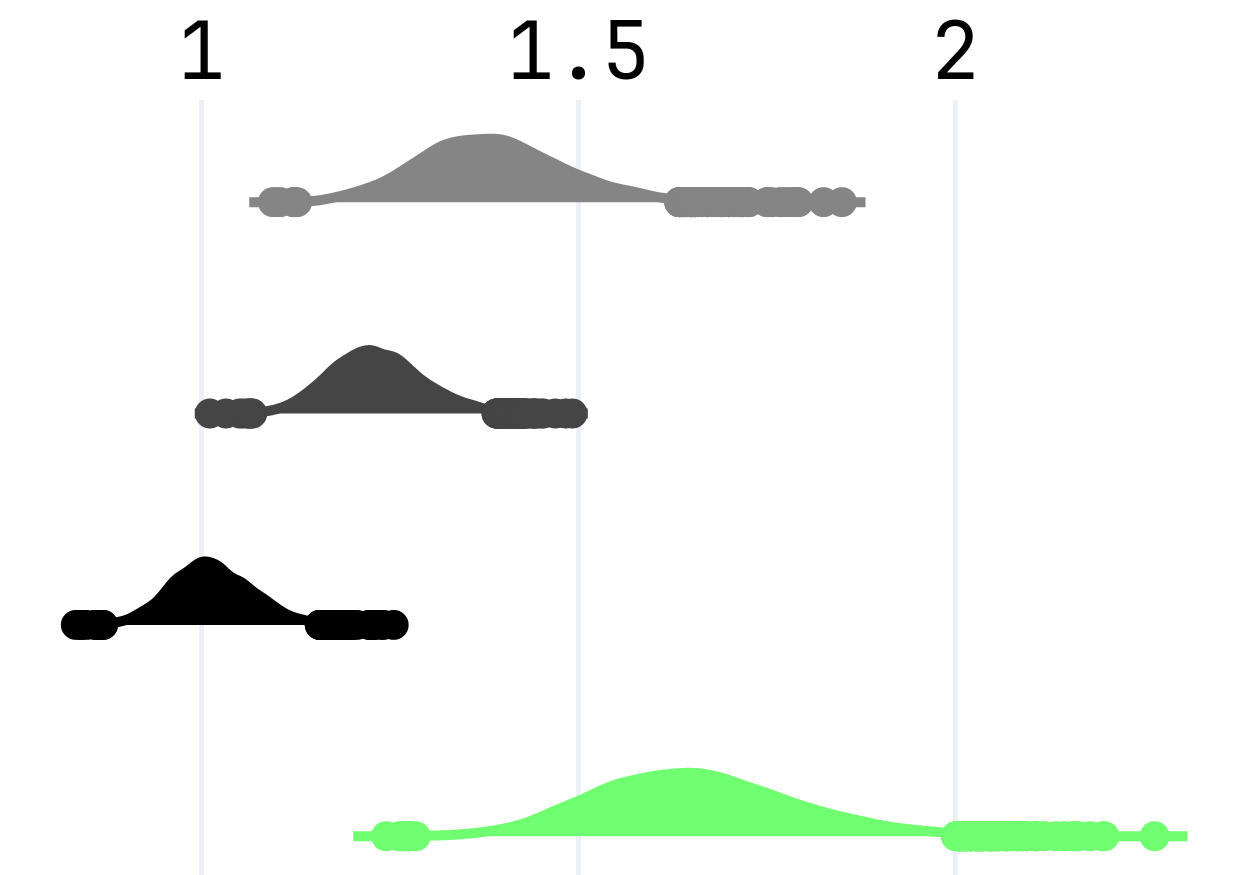
\includegraphics[width=\linewidth]{images/npsk_ood_P_Loss_0.png}
        \vspace{0.3em}
        \footnotesize (a)~Non-Overlapping Frequencies
      \end{minipage}
      \hspace{0.015\textwidth}%
      \begin{minipage}[t]{0.31\textwidth}
        \centering
        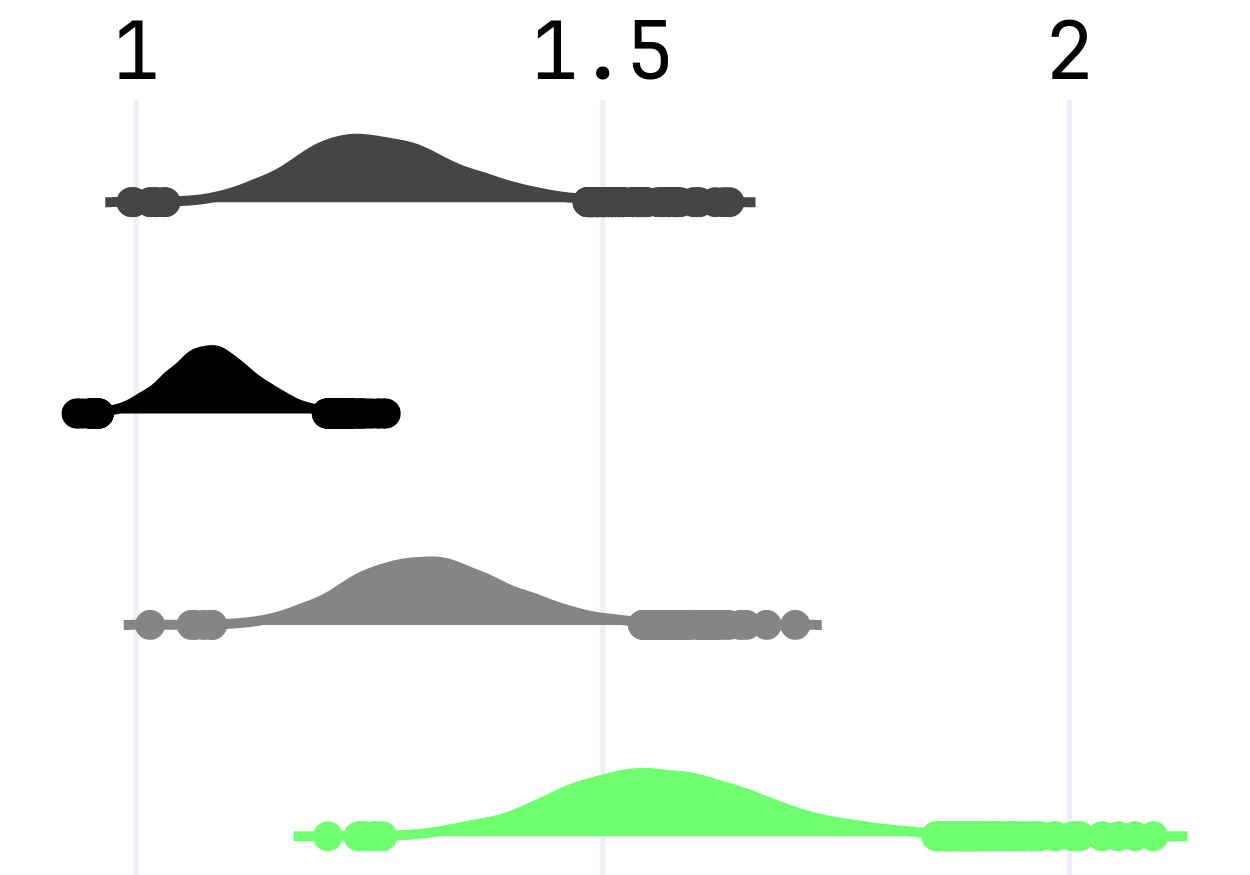
\includegraphics[width=\linewidth]{images/npsk_ood_P_Loss_1.png}
        \vspace{0.3em}
        \footnotesize (b)~Sine Target, Saw Imitator
      \end{minipage}
      \hspace{0.015\textwidth}%
      \begin{minipage}[t]{0.31\textwidth}
        \centering
        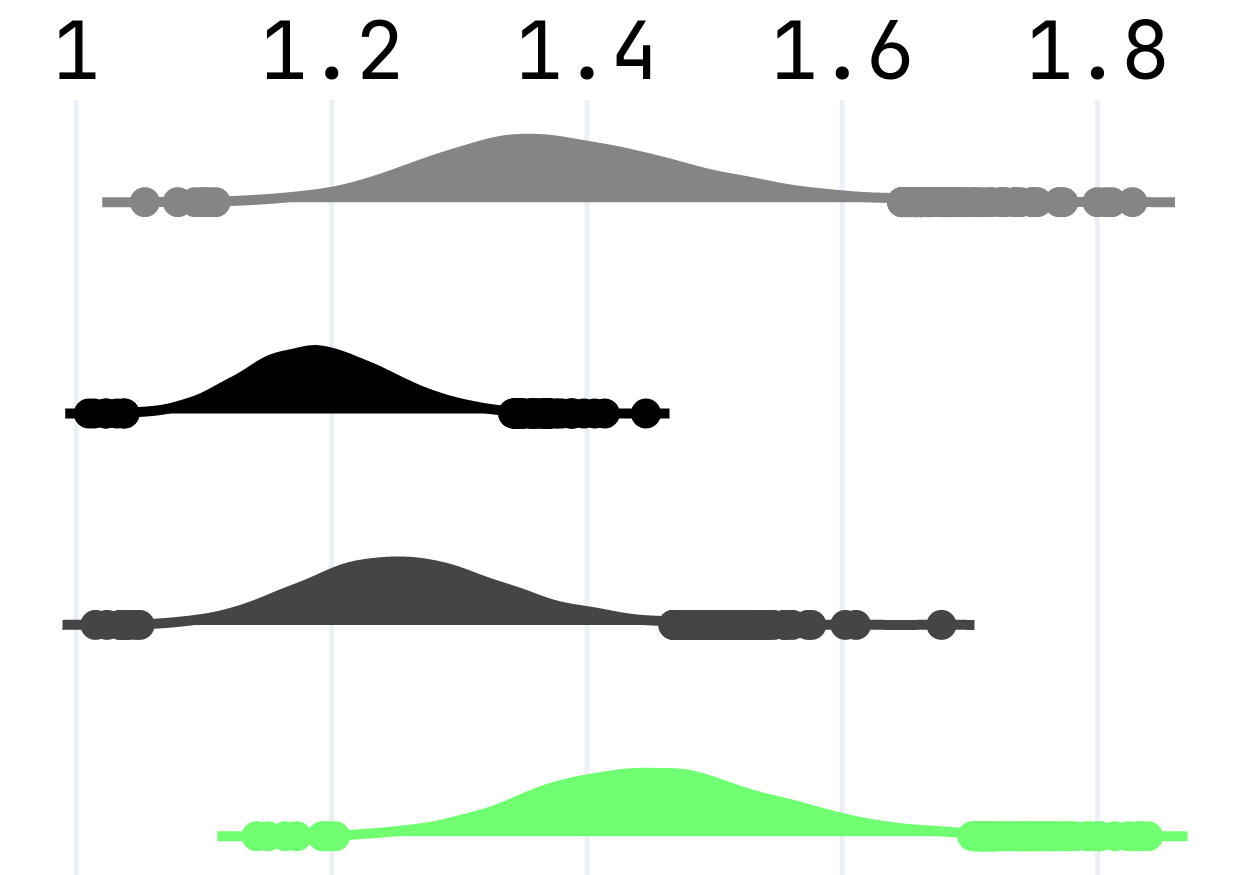
\includegraphics[width=\linewidth]{images/npsk_ood_P_Loss_2.png}
        \vspace{0.3em}
        \footnotesize (c)~Saw Target, Sine Imitator
      \end{minipage}
    \end{minipage}
  \end{minipage}
  \caption{Bootstrapped distributions and ranks for AM-Synthesizer sound matching.}
  \label{fig:npsk_am_synths}
\end{figure*}


\begin{figure*}[t]
  \centering
  \begin{minipage}[t]{\textwidth}
    % Left-side labels
    \begin{minipage}[t]{0.045\textwidth}
      \footnotesize\raggedleft
      \vspace{-3cm} % align with top of images
      SIMSE\\[0.4cm]
      L1\\[0.385cm]
      JTFS\\[0.365cm]
      DTW
    \end{minipage}%
    \hspace{0.01\textwidth}%
    % Right side: images + captions
    \begin{minipage}[t]{0.91\textwidth}
      \centering
      \begin{minipage}[t]{0.31\textwidth}
        \centering
        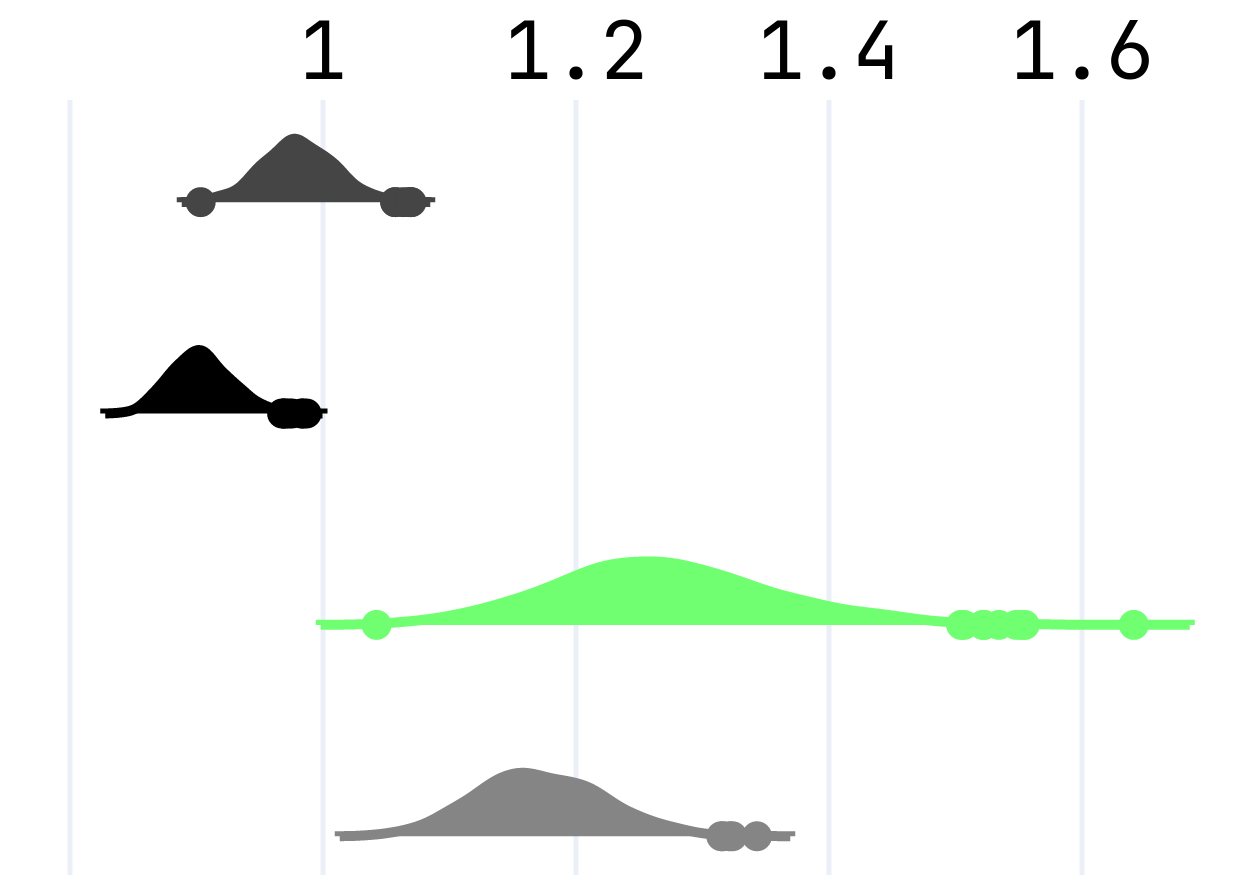
\includegraphics[width=\linewidth]{images/npsk_ood_P_Loss_4.png}
        \vspace{0.3em}
        \footnotesize No-delay Pitch-bend
      \end{minipage}
      \hspace{0.015\textwidth}%
      \begin{minipage}[t]{0.31\textwidth}
        \centering
        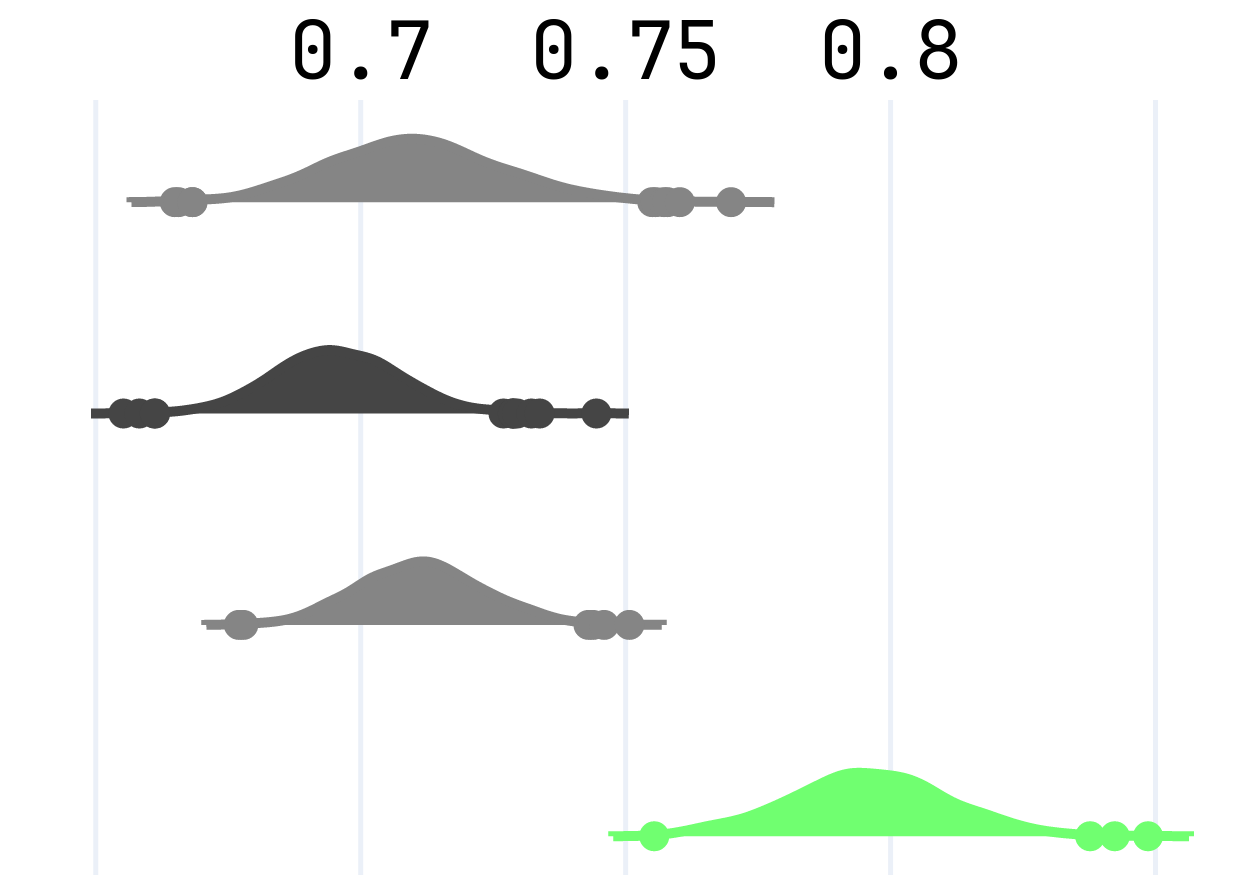
\includegraphics[width=\linewidth]{images/npsk_ood_P_Loss_5.png}
        \vspace{0.3em}
        \footnotesize Pulsating Pitch-bend
      \end{minipage}
            \hspace{0.015\textwidth}%
      \begin{minipage}[t]{0.31\textwidth}
        \centering
        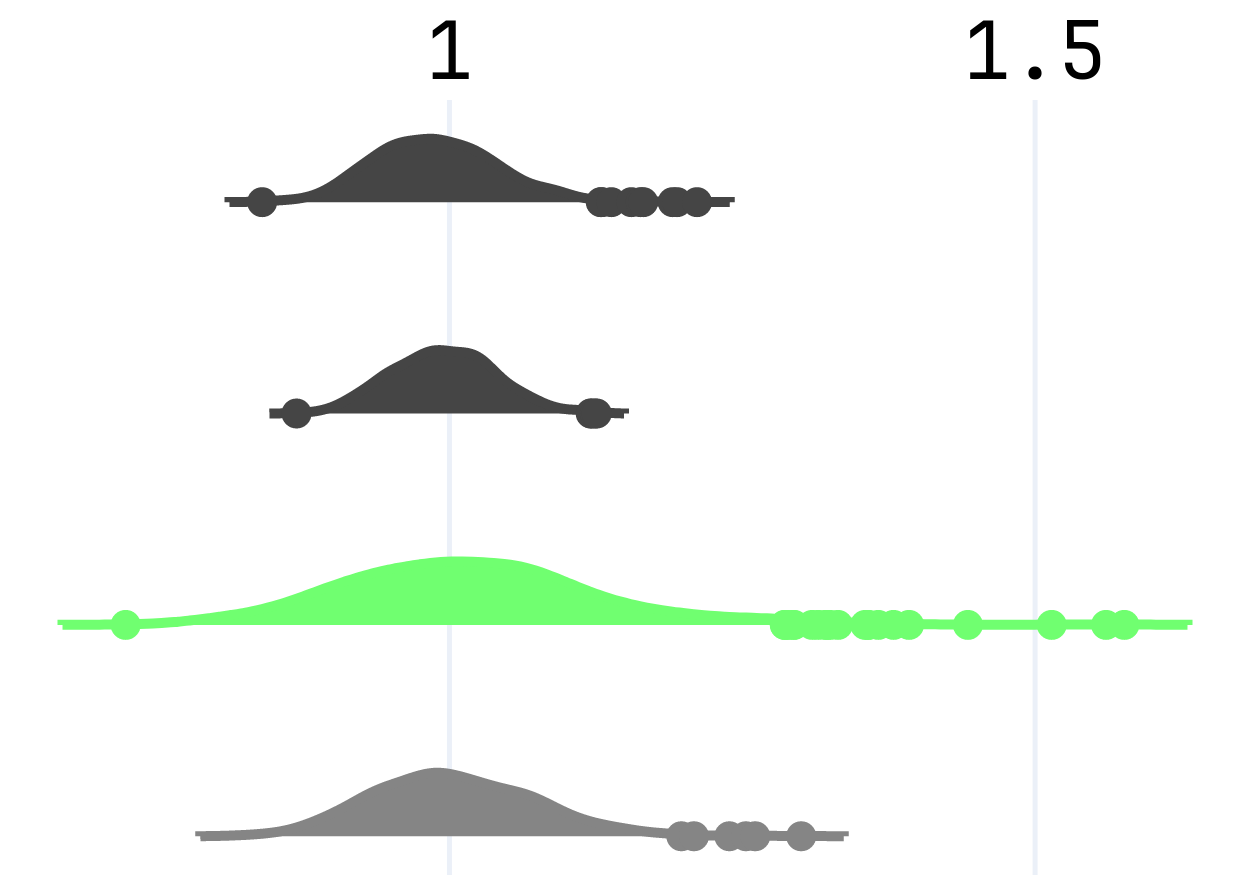
\includegraphics[width=\linewidth]{images/npsk_ood_P_Loss_6.png}
        \vspace{0.3em}
        \footnotesize Delayed Pitch-Bend
      \end{minipage}
    \end{minipage}
  \end{minipage}
  \caption{Bootstrapped distributions and ranks for non-delayed and randomly delayed pitch-bend programs.}
  \label{fig:npsk_pitch-bends}
\end{figure*}

\subsection{Delayed Pitch-Bending}
In this scenario, we create a synthesizer that replicates some of the key characteristics of a chirplet synthesizer~\cite{vahidi2023mesostructures} \todo{which does what?}. The program here is a sine wave with a steady starting pitch for a random amount of time; after a time delay of 5000-30000 samples (the sampling rate is set to 48000), an exponential upward pitch bend is applied to the starting pitch. The search parameters here are the starting pitch (30-500 Hz) and the rate at which the power of the exponent increases (1-20 samples at every time step). The time-delay for the pitch-bending onset is selected randomly for each experiment, so it is very unlikely that the imitator would be able to replicate the target's sounds, making this an out-of-domain example.

Here, we can define success with P-Loss, that is, how well the \texttt{increase\_speed} and \texttt{starting\_pitch} parameters are approximated despite the delay in the pitch-bending onset. Figure~\ref{fig:npsk_pitch-bends} the right side shows that \JTFS is the best performing loss function, which is consistent with the previous findings by Vahidi \textit{et al.}~\cite{vahidi2023mesostructures}. 

An interesting follow-up experiment conducted was the \textit{in-domain} comparison of pitch-bending synthesizers \textit{without} delay. This is identical to the delayed pitch-bending experiment but setting the delay variable $\delta=0$. The left side of Figure~\ref{fig:npsk_pitch-bends} shows that \DTWEnv is the better performer in the in-domain scenario.

\begin{lstlisting}[escapeinside={(*}{*)},caption={\PitchBendUp program. when an instance of the synthezier is created, $\delta$ is randomly assigned a value between 5000-30000 samples}, label={lst:pitchbendup},language=Faust,float,floatplacement=!H,xleftmargin=1em,xrightmargin=0.5em,firstnumber=0,aboveskip=0em, belowskip=-1em]
import("stdfaust.lib");
increase_speed = hslider("increase_speed",2,1,20,0.1);
starting_pitch = hslider("starting_pitch",200,30,500,0.1);
sineOsc(f) = +(f/ma.SR) ~ ma.frac:*(3*ma.PI):sin;
increasing_pitch(rate) = _ ~+(rate/ma.SR):exp;
process = sineOsc(increasing_pitch(increase_speed):de.delay((*$\delta$*),48000)+starting_pitch);

\end{lstlisting}

\section{Gradients}
Different forms of gradient analysis has been conducted in previous works~\cite{masuda2023improving,turian2020sorry,vahidi2023mesostructures}.


\section{Conclusion and Summary}
We presented different out-of-domain sound-matching scenarios, and saw that the success of the loss functions was highly dependent on the method of synthesis. This further solidifies our previous work which advocated against the search for a universally optimal loss function for sound~\cite{salimi2025soundmatching}.

\clearpage
\bibliographystyle{alpha}
\bibliography{references}

\end{document}
